\documentclass{article}
\usepackage{geometry}

\geometry{a4paper,left=2cm,right=2cm,top=1cm,bottom=1.25cm}
\usepackage{xeCJK, fontspec, xunicode, xltxtra}  
\usepackage[colorlinks,
            linkcolor=blue,
            anchorcolor=blue,
            citecolor=blue
            ]{hyperref}
%\setCJKmainfont{Hiragino Sans GB}  
\setmainfont{Times New Roman}  
\setCJKmainfont{Songti SC}

\usepackage{graphicx} 
\usepackage{amsmath}
\usepackage{amssymb}

\usepackage{listings}
\usepackage{xcolor}
\lstset{
    numbers=left, 
    numberstyle= \tiny, 
    keywordstyle= \color{ blue!70},
    commentstyle= \color{red!50!green!50!blue!50}, 
    frame=shadowbox, % 阴影效果
    rulesepcolor= \color{ red!20!green!20!blue!20} ,
    escapeinside=``, % 英文分号中可写入中文
    xleftmargin=2em,xrightmargin=2em, aboveskip=1em,
    framexleftmargin=2em
} 


\title{Report of Assignment 7}
\author{Haodong Liao \& Liyuan Zhang}

\begin{document}
\maketitle{}

% \quad Having changed the class of Coursera course : Interactive Computer Graphics by Takeo Igarashi of The University of Tokyo to June 25, I have to wait until then. And due to the final exam of 3D Graphic Programming, I didn't get the time to study the Coursera course : Introduction to C\# Programming and Unity by  Dr. Tim "Dr. T" Chamillard of The University of Colorado either.

% \section{The tasks I have done last week}
% \begin{itemize}%项目符号开始

% %\item Having changed the class of Coursera course : Interactive Computer Graphics by Takeo Igarashi of The University of Tokyo to June 25, I have to wait until then. And due to the final exam of 3D Graphic Programming, I didn't get the time to study the Coursera course : Introduction to C\# Programming and Unity by  Dr. Tim "Dr. T" Chamillard of The University of Colorado either.

% %\item I've submited my curriculum design.

% %\item I'm studying a Coursera course:Introduction to C\# Programming and Unity by  Dr. Tim "Dr. T" Chamillard of The University of Colorado,and finished the study of Week 1.

% %\item I've taken the final exam of the mathematical modeling course.

% %\item I'm participated in the summary defense of the student union of the youth league committee of the school of computer science and engineering.

% \item I have been reviewing the final exam of 3D Graphic Programming.


% \end{itemize}

% \section{My plan for next week}

% \noindent
% \qquad I plan to do things as follows:

% \begin{itemize}

% \item Finish the Week2 course of Introduction to C\# Programming and Unity by  Dr. Tim "Dr. T" Chamillard of The University of Colorado

% \item Review the final exam of Database.
% \item Review the final exam of Computer Network.
% \item Review the Rebuilt test of Calculus 1 \& 2.

% \end{itemize}

\section{Preface}

This was a \LaTeX report written by Haodong Liao and Liyuan Zhang, students of UESTC who participated in the summer school of UCPH. More codes of this summer school were at this \href{https://github.com/Medill-East/ComputerScience/tree/master/Professional%20Core%20Courses/Functional%20Programming/SummerSchool}{repository}.

\section{Introduction}

A string in F\# was a sequence of characters\footnote[1]{https://docs.microsoft.com/en-us/dotnet/fsharp/language-reference/lists}, and some of the string functions were similar to list functions, after the practicing of the list function, it was time to move on.

In this assignment, we worked with simple text processing and met the requirements of analyzing and generating some text according to statistics. In detail, we used pattern-matching and explicit type definition to create our own recursive functions, besides, we used powerful List-library functions to read, convert, analyze and generate target text.

% All in all, the results I achieved were as following:

% \begin{itemize}
% \item met the requirement of replacing the library calls in \emph{myFold} and \emph{myFilter} with my own recursive implementations of these functions,
% \item used \emph{match..with} to achieved pattern-matching,
% % \item made the program work on my own and improved \emph{myFold} function to be more generic with the help of Prof.Sporring.
% \end{itemize}

% The remaining structure of the article is as follows. Section 3 states the problem in detail. Section 4 analysis and designs the problem. Section 5 describes the essential parts of my implementation. The program is evaluated in Section 6 and discussed in Section 7.

% \section{Problem statement}

% This assignment required us to replace the library function with recursive implementations for \emph{myFold} and \emph{myFilter} based on the file \emph{recursiveMapFoldFilter.fsx}, which is a fully functioning program must be compiled and executed from the console. 

% This program takes 2 arguments: a string and a positive integer \emph{n}. The string can be either \emph{map}, \emph{fold}, or \emph{filter}. The output is a random list of length \emph{n} consisting of positive integers less than 10 and a processed list. For \emph{fold}, the random elements have been multiplied by 2 and their order has been reversed, and for \emph{filter}, only those elements larger than 4 have been included.

\section{Analysis and Design}

\subsection{Text Processing of character}
\subsubsection{ReadText}
% \lstset{language=Csh}
\begin{lstlisting}
readText: filename:string -> string
// readFile.fsx
let filename = "readFile.fsx"
let line = 
  try
    let reader = System.IO.File.OpenText filename
    reader.ReadToEnd ()
  with
    _ -> "" // The file cannot be read, so we return an empty string
printfn "%s" line
\end{lstlisting}

In this sub-assignment, we needed to convert \emph{readFile.fsx} into a more flexible function which reads the content of any text file.

Referred to the input processing code in assignment 6, there were two branches needed to be handled, one was to set the entry point of our code, the other was to change the fixed argument to a flexible one so that the function could read the content of any text file. The key part of the pseudocode was shown as following:

\begin{lstlisting}
[<EntryPoint>]
let main (input argument) = 
  if (argument correct)
    call readText function with responding name of file    
  else
    display error message
\end{lstlisting}

\subsubsection{ConvertText}
% \lstset{language=Csh}
\begin{lstlisting}
convertText: src:string -> string
\end{lstlisting}

The goal of this sub-assignment was to convert letters of a string to lower case and removes all characters except a..z. 
According to \cite{sporring2019}, there was a \emph{ToLower()} function \emph{returns a copy of the string where each letter has been converted to lower case}, so we could use it to finish the 'convert' part and moved on to 'remove' part. The key part of the pseudocode is shown as following:

\begin{lstlisting}
let convertText inputString = 
  let lowerStr = inputString.ToLower()
    if (elment of lowerStr was in the range of a..z)
      keep the current element
    else remove the current element  
\end{lstlisting}

\subsubsection{Get Histogram}
% \lstset{language=Csh}
\begin{lstlisting}
histogram: src:string -> int list
\end{lstlisting}

We needed to count occurrences of each lower-case letter of the English alphabet in a string and returned a list in this sub-assignment. According to \cite{sporring2019}, there was a \emph{String.filter} function similar to \emph{List.filter} function, we used it to filter the specific letter of the string and count the length of it to get the occurrences. The key part of the pseudocode was shown as following:

\begin{lstlisting}
let countchar (src:string)(letter:char) = 
      if letter was in the range of a..z then 
        filter the current letter
        handle the rest string
      else
        returned an empty list
let histogram (src:string): int list = (countchar src 'a')
\end{lstlisting}

\subsubsection{Generate Ramdom String}
% \lstset{language=Csh}
\begin{lstlisting}
randomString: hist:int list -> len:int -> string
\end{lstlisting}

The requirement of this sub-assignment was to change the given program and generate a string of a given length and contained random characters distributed according to a given histogram which used our own functions. The flow of the program was shown as following:

\begin{lstlisting}
step1 - Read the target text file and saved it
step2 - Converted the text to lower case & removed characters except a..z
step3 - Got the histogram of the text
step4 - Generated a new random string according to the histogram
\end{lstlisting}

\subsection{Text Processing of pair of characters}

\subsubsection{Get Cooccurrence}

In this sub-assignment, we needed to count occurrences of each pair of lower-case letter of the English alphabet in a string and return a list of lists. Our solution was to use double recursion and process the letter in each pair separately. The key part of the pseudocode was shown as following:

\begin{lstlisting}
// count the occurrence of each pair
let countnum = 
  if the length of src > 2 then
    if the first two char = charpair then
      1 + sum recursively
    else
      ignore current and sum recursively
  else
    return 0      
// handle the second letter    
let countcharpair = 
  if the second letter <= 'z' then
    sum the occurrence and process the left string recursively
  else return an empty list   
// process the first letter
let countchar = 
  if the first letter <= 'z' then
    process the second letter and process the left string recursively
  else return an empty list    
// call function from here
let cooccurrence (src:string) = countchar src 'a'
\end{lstlisting}

\subsubsection{Markov Model}
% \lstset{language=Csh}
\begin{lstlisting}
fstOrderMarkovModel: cooc: int list list -> len:int -> string
\end{lstlisting}

We needed to generate a random string of length \emph{len}, whose character pairs were distributed according to a specified cooccurrence histogram \emph{cooc} of the story "Little Claus and Big Claus" in this sub-assignment. The flow of the program was shown as following:

\begin{lstlisting}
step1 - Count the occurrence of each pairs (like 'aa' to 'az')
step2 - Count the coocurrence of all pairs ('aa' to 'zz')
step3 - Calculate the ratio of each pairs
step4 - Generate a random string of length len
  according to a given cooccurrence and the ratio of each pairs
\end{lstlisting}


\section{Program description}

Our implementation of \textbf{readText} function was as follows:

\begin{lstlisting}
let printErrorMessage () =
    printfn "Program Input should be 'readfile filename'"

let readText (filename:string) : string = 
    let line = 
        try
          let reader = System.IO.File.OpenText filename
          reader.ReadToEnd ()
        with
          _ -> "" // The file cannot be read, so we return an empty string
    printfn "%s" line
    line
[<EntryPoint>]
let main (paramList : string[]) : int = 
    if paramList.Length <> 2 then
        printErrorMessage ()
        0
    else
        match paramList.[0] with
            | "readfile" ->
                let str = readText paramList.[1]
                printfn "str : %A" str
            | _ ->
                printErrorMessage ()
        1    
\end{lstlisting}

As it showed, the key to this function was to match the argument list, the first argument should be the command 'readfile', and the second argument was the name of a  file.

Implementation of \textbf{convertText} function was as follows:

% \lstset{language=Csh}
\begin{lstlisting}
let rec convertText (src:string) : string = 
    let lowerSRC = src.ToLower()
    match lowerSRC with
    | "" -> ""
    | elm -> 
        if ('a' <= elm.[0] && elm.[0] <= 'z')
        then 
            elm.[0].ToString() + (convertText elm.[1..])
        else
            convertText elm.[1..]
\end{lstlisting}

It made us wondering whether there was an expression of string could work as 'elm::rest' to represent a list at the beginning, things did not go well so we changed our mind to use elm[1..] to represent the rest of a string.

Implementation of \textbf{histogram} function was as follows:

% \lstset{language=Csh}
\begin{lstlisting}
let rec countchar (src:string)(letter:char): int list = 
  if letter >= 'a' && letter <= 'z' then 
    ((String.filter (fun char -> char=letter) src).Length)::
     (countchar src (char (int letter + 1)))
  else []
let histogram (src:string): int list = (countchar src 'a')
\end{lstlisting}

This function was the key to solving the following problems.

\textbf{Assignment 7.4} was a summary of the previous assignments, and the key part to it was as follows:
% \lstset{language=Csh}
\begin{lstlisting}
/// step1 readfile
let str = readText "littleClausAndBigClaus.txt"
/// step2 convertfile
let convertRes = convertText str
/// step3 get histogram
let hist = histogram convertRes
let alphabet = List.init hist.Length (fun i -> 'a' + char i)
printfn "A histogram:\n %A" (List.zip alphabet hist)
/// step4 generages a new random string
let ranStr = randomString hist convertRes.Length
printfn "A random string: %s" ranStr
let newHist = histogram ranStr
printfn "Resulting histogram:\n %A" (List.zip alphabet newHist)
\end{lstlisting}

It was important to have a clear thought of processing flow.

Implementation of \textbf{cooccurrence} function was as follows:

% \lstset{language=Csh}
\begin{lstlisting}
let rec countnum (src:string) (charpair:string):int =
  if src.Length >=2 then
    if src.[0..1] = charpair then
      1+(countnum src.[1..] charpair)
    else
      (countnum src.[1..] charpair)
  else
    0
let rec countchapair (src:string) (letter1:char) (letter2:char):int list =
  if letter2 <= 'z' then
    let charpair = string letter1 + string letter2
    (countnum src charpair)::(countcharpair src letter1 (letter2+char 1))
  else []
let rec countchar (src:string) (letter1:char):int list list = 
  if letter1 <= 'z' then
    (countcharpair src letter1 'a')::(countchar src (letter1 + char 1))
  else []
let cooccurrence (src:string):int list list =
  countchar src 'a'
\end{lstlisting}

This was a difficult problem for us, and the key to the solution was the idea of 'divide and conquer'. If we could not process the pair of letters at a time, we handle the letter of it separately.

\textbf{Assignment 7.6} was a summary of all the previous assignments, and the key part of the implementation of it was as follows:
% \lstset{language=Csh}
\begin{lstlisting}
let fstOrderMarkovModel (cooc:int list list) (len:int):string =
    let strLengthlist = 
      List.map (fun x -> (float x)) (List.map (List.sum) cooc)
    let strLengthSum = List.sum strLengthlist
    let ratiolist = List.map (fun x -> x/strLengthSum) strLengthlist
    let randomStringAlt (hist: int list):string = randomString hist 
      (int((float (List.sum (hist))/strLengthSum)*(float len)))
    let strlist = List.map (randomStringAlt) cooc
    let composestr (acc:string) (elm:string):string = acc + elm
    List.fold composestr "" strlist
printfn "test: \n %A" (fstOrderMarkovModel (cooccurrence a) (a.Length))
printfn "present cooc : \n %A" 
  (cooccurrence (fstOrderMarkovModel (cooccurrence a) (a.Length)))
\end{lstlisting}

This was another difficult assignment for us, the main challenge was to arrange the text properly so the occurrence was similar. We tried to generate a new character according to the letter before the current letter, but things just did not work well for reason we did not figure out, then we tried with the weight of the pair based on the proportion of the sum of the single letters to the sum of the occurrences of all the letters
 % for example:
% \begin{math}
% $$Weight_{'a..'} = \frac{Occurrence of 'aa' to 'az'}{Occurrence of 'aa' to 'zz'}$$
% \end{math}
. In this way, when there was a given length, the length of each character list (like 'aa'..'az') would be its weight timed the given length, such as:
\begin{math}
$$Length_{'aa'to'az'} = \frac{Occurrence_{'aa' to 'az'}}{Occurrence_{'aa' to 'zz'}} * (Given Length)$$
\end{math}
, so that we could generate a random string which had a similar distribution but different content.

\section{Evaluation}

The testing environment was macOS Mojave 10.14.5 system with iTerm and Microsoft (R) F\# Compiler version 4.1.

We combined all the assignment into a single program, compiled and tested it with parameter \emph{readfile littleClausAndBigClaus.txt}. Output of it included \emph{content of target file}, \emph{converted string of original string}, \emph{histogram of original string}, \emph{random string of single character}, \emph{histogram of random single character}, \emph{cooc of original string}, \emph{cooc of random single character}, \emph{random string of character pairs} and \emph{cooc of random character pairs}. Part of results (because it was too long) were shown as following (the complete results could be seen at \href{https://github.com/Medill-East/ComputerScience/blob/master/Professional%20Core%20Courses/Functional%20Programming/SummerSchool/Learning%20Material/Report/Hand-in/2/Result/Result.txt}{result}):

\begin{figure}[htbp]
      \centering
      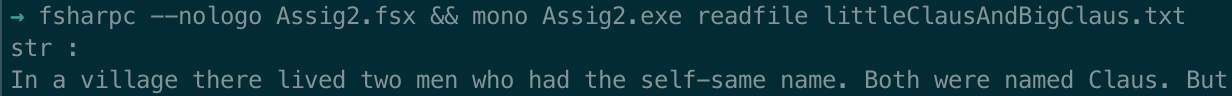
\includegraphics[width=\linewidth]{inputandread}
      \caption{Testing of readText function}
      \label{fig:inputandread}
\end{figure}

% \begin{figure}[htbp]
%       \centering
%       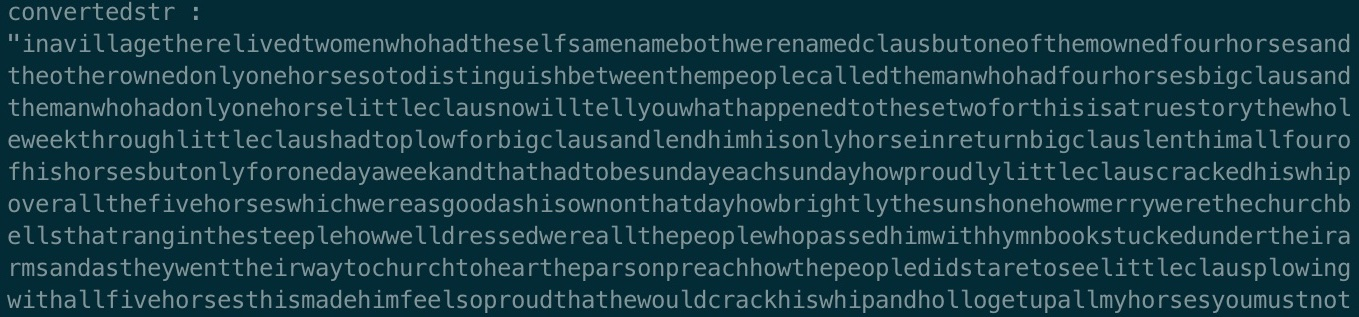
\includegraphics[width=\linewidth]{convert}
%       \caption{Testing of convertText function}
%       \label{fig:convert}
% \end{figure}

% \begin{figure}[htbp]
%       \centering
%       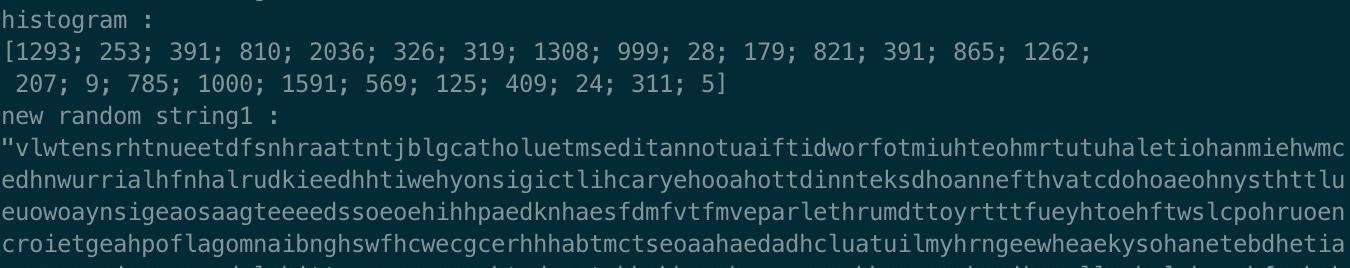
\includegraphics[width=\linewidth]{histogramandnewstring1}
%       \caption{Testing of histogram and randomString function}
%       \label{fig:histogramandnewstring1}
% \end{figure}

% \begin{figure}[htbp]
%       \centering
%       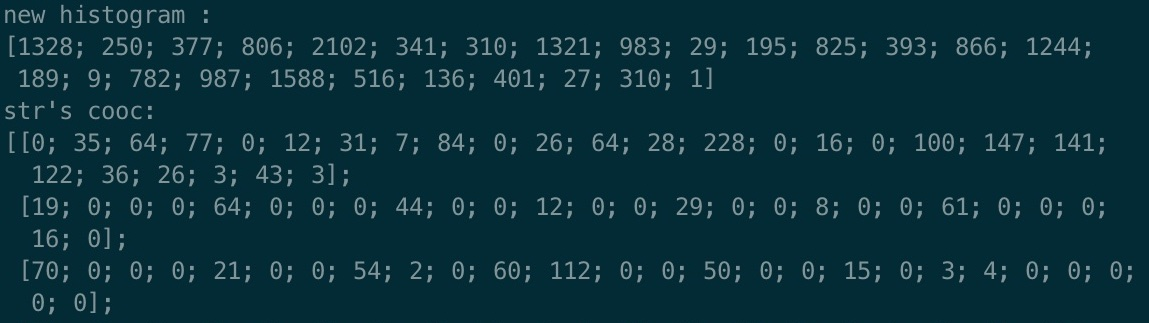
\includegraphics[width=\linewidth]{newhistogram1andoldcooc}
%       \caption{Histogram and Cooc of Generate String of randomString function}
%       \label{fig:newhistogram1andoldcooc}
% \end{figure}

\begin{figure}[htbp]
      \centering
      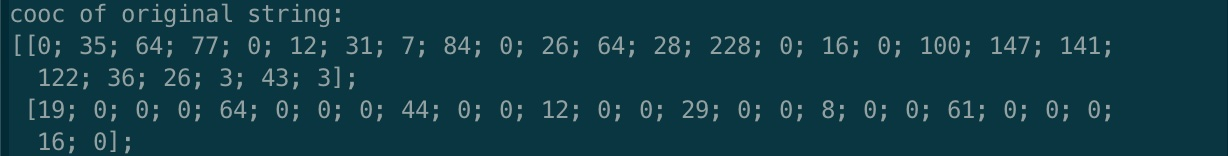
\includegraphics[width=\linewidth]{coocoforiginalstring}
      \caption{Testing of fstOrderMarkovModel function}
      \label{fig:coocoforiginalstring}
\end{figure}

\begin{figure}[htbp]
      \centering
      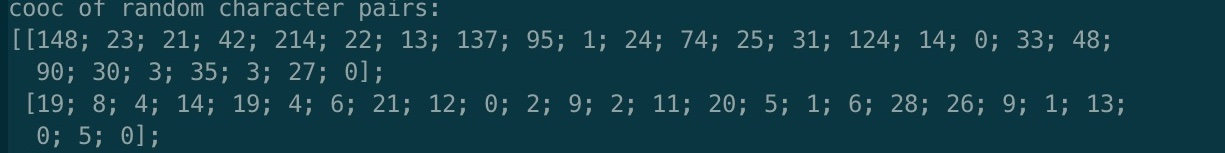
\includegraphics[width=\linewidth]{coocofcharacterpairs}
      \caption{Coocurrence of fstOrderMarkovModel function}
      \label{fig:coocofcharacterpairs}
\end{figure}

\section{Conclusion}

In this assignment, we worked with simple text processing and met the requirements of analyzing and generating target text according to statistics. It was time-consuming of thinking about the recursive function and avoiding to use things like 'for loop' when we were stuck, it was challenging but this assignment made us get more familiar with F\# and functional programming indeed. It was our pleasure to have teachers like Prof.Sporring and we believed that we had a good time. Many thanks!


%\renewcommand\refname{Reference\\
%\small those are reference form Week 6, I'll list Week5's reference next time}
\bibliographystyle{unsrt}
\bibliography{reference}

%\begin{thebibliography}{99}
%\bibitem{1} \href{http://research.nii.ac.jp/~takayama/metallophone/metallophone-cga2011.pdf}{Responsive FEM for Aiding Interactive Geometric Modeling} \\
%Umetani N, Takayama K. Responsive FEM for Aiding Interactive Geometric Modeling[J]. 2010.

%\bibitem{2} \href{http://www-ui.is.s.u-tokyo.ac.jp/~takeo/papers/umetani_nime2010_metallophone.pdf}{Designing Custom-made Metallophone with Concurrent Eigenanalysis}\\
%Umetani N, Mitani J, Igarashi T. Designing Custom-made Metallophone with Concurrent Eigenanalysis[J]. Data, 2010. 

%\bibitem{3} \href{http://www.jst.go.jp/erato/igarashi/publications/001/SensitiveCouture.pdf}{Sensitive Couture for Interactive Garment Modeling and Editing}\\
%Umetani N, Kaufman D M, Igarashi T, et al. Sensitive couture for interactive garment modeling and editing[C]// ACM, 2011:1-12.

%\bibitem{4} \href{http://www.jst.go.jp/erato/igarashi/en/projects/GuidedExploration/2012_siggraph_GuidedExploration.pdf}{Guided Exploration of Physically Valid Shape for Furniture Design}\\
%Umentani N, Igarashi T, Mitra N J. Guided exploration of physically valid shapes for furniture design[J]. Communications of the ACM, 2015, 58(9):116-124.

%\bibitem{5} \href{http://www.nobuyuki-umetani.com/publication/2014_sigg_pteromys/2014_siggraph_GliderDesign.pdf}{Pteromys: Interactive Design and Optimization of Free-formed Free-flight Model Airplanes}\\
%Umetani N, Koyama Y, Schmidt R, et al. Pteromys:interactive design and optimization of free-formed free-flight model airplanes[J]. Acm Transactions on Graphics, 2014, 33(4):1-10. 

%\bibitem{6} Mori Y, Igarashi T. Plushie: an interactive design system for plush toys[C]//ACM Transactions on Graphics (TOG). ACM, 2007, 26(3): 45.

%\bibitem{7} Igarashi Y, Igarashi T, Mitani J. Beady: interactive beadwork design and construction[J]. ACM Transactions on Graphics (TOG), 2012, 31(4): 49.
 
%\bibitem{8} Saul G, Lau M, Mitani J, et al. SketchChair: an all-in-one chair design system for end users[C]//Proceedings of the fifth international conference on Tangible, embedded, and embodied interaction. ACM, 2011: 73-80.
 
%\bibitem{9} Saakes D, Cambazard T, Mitani J, et al. PacCAM: material capture and interactive 2D packing for efficient material usage on CNC cutting machines[C]//Proceedings of the 26th annual ACM symposium on User interface software and technology. ACM, 2013: 441-446.

% \bibitem{10} A. Rovira, D. Swapp, B. Spanlang, and M. Slater. The use of virtual reality in the study of people’s responses to violent incidents. Frontiers in Behavioral Neuroscience, 3(59), 2009. doi: 10.3389/neuro.08.059.2009
 %\bibitem{11} J.Russell.Agency:itsroleinmentaldevelopment.EssaysinEnvironmen- tal Psychology. Psychology Press, East Sussex, UK, 1996.
 %\bibitem{12} R.Skarbez.Apreliminaryinvestigationofplaceillusionandplausibility illusion. In IEEE Virtual Reality (VR) Doctoral Consortium, 2015.
 %\bibitem{13} M.Slater.Placeillusionandplausibilitycanleadtorealisticbehaviorin immersive virtual environments. Philosophical transactions of the Royal Society of London. Series B, Biological sciences, 364:3549–3557, 2009.
 %\bibitem{14} M. Slater, P. Khanna, J. Mortensen, and I. Yu. Visual realism enhances realistic response in an immersive virtual environment. IEEE Computer Graphics and Applications, 29:76–84, 2009. doi: 10.1109/MCG.2009.55
 %\bibitem{15} M. Slater, B. Spanlang, and D. Corominas. Simulating virtual environ- ments within virtual environments as the basis for a psychophysics of presence. ACM Trans. Graph., 29:92:1–92:9, July 2010. doi: 10.1145/ 1778765.1778829
 
%\end{thebibliography}



\end{document}